The Recipe Approximation Problem (RAP) was originally conceived by Kyle Oliver
in \cite{oliver_geniusv2:_2009}. It was the result of conversations with
scientists of the VISION fuel cycle simulation team \cite{vision2009} with what
was then called the Winery Problem, because of the similarity due to mixing
vintages of win to match a given recipe. This work expands Oliver's initial
formulation by correcting an error and expanding the single-request formulation
to an N-request formulation.

The Recipe Approximation Problem (RAP) seeks to model a separations facility
matching reactor fuel orders. The basic assumptions of the problem are the
following: there are a set of barrels of separated material, $B$, and a set of
fuel requests, $R$, that specify an isotopic vector, $I_{r}$, and quantity,
$q_{r}$, that fully describe a desired fuel order. The goal of the solution
methodology is to determine a matrix of extraction fractions $X$, where each
entry, $x_{b,r}$ denotes the fraction of barrel $b$ being used to match fuel
request $r$. The problem is shown graphically in Figure \ref{fig:rap},
displaying the set of barrels, $B$, the set of fuel requests, $R$, and the set
of extraction fractions, $X$.

\begin{figure}[h]
  \begin{center}
    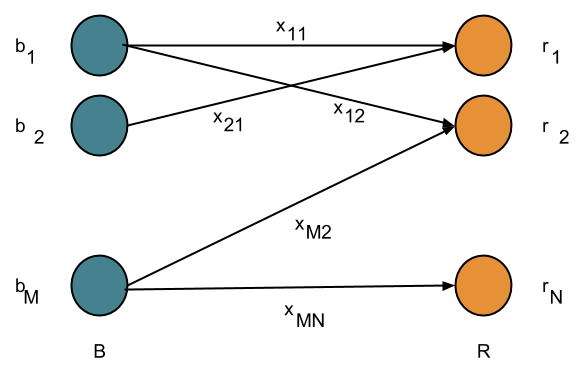
\includegraphics[width=8cm]{./chapters/research/rap.png}
  \caption{A graphical view of an example solution to the Recipe Approximation 
           Problem.}
  \label{fig:rap}
  \end{center}
\end{figure}

The optimal extraction fractions are modeled as the solution to an
approximation linear program, the foundations of which were described in
\S\ref{sec:approx}. Below I describe the most straightforward formulation of 
the RAP, expanding upon the work in \cite{oliver_geniusv2:_2009}. I then
describe how additional constraints can be added to the formulation given
additional information. Finally, I describe a more abstract version that adds a
notion of agency to the problem formulation.

